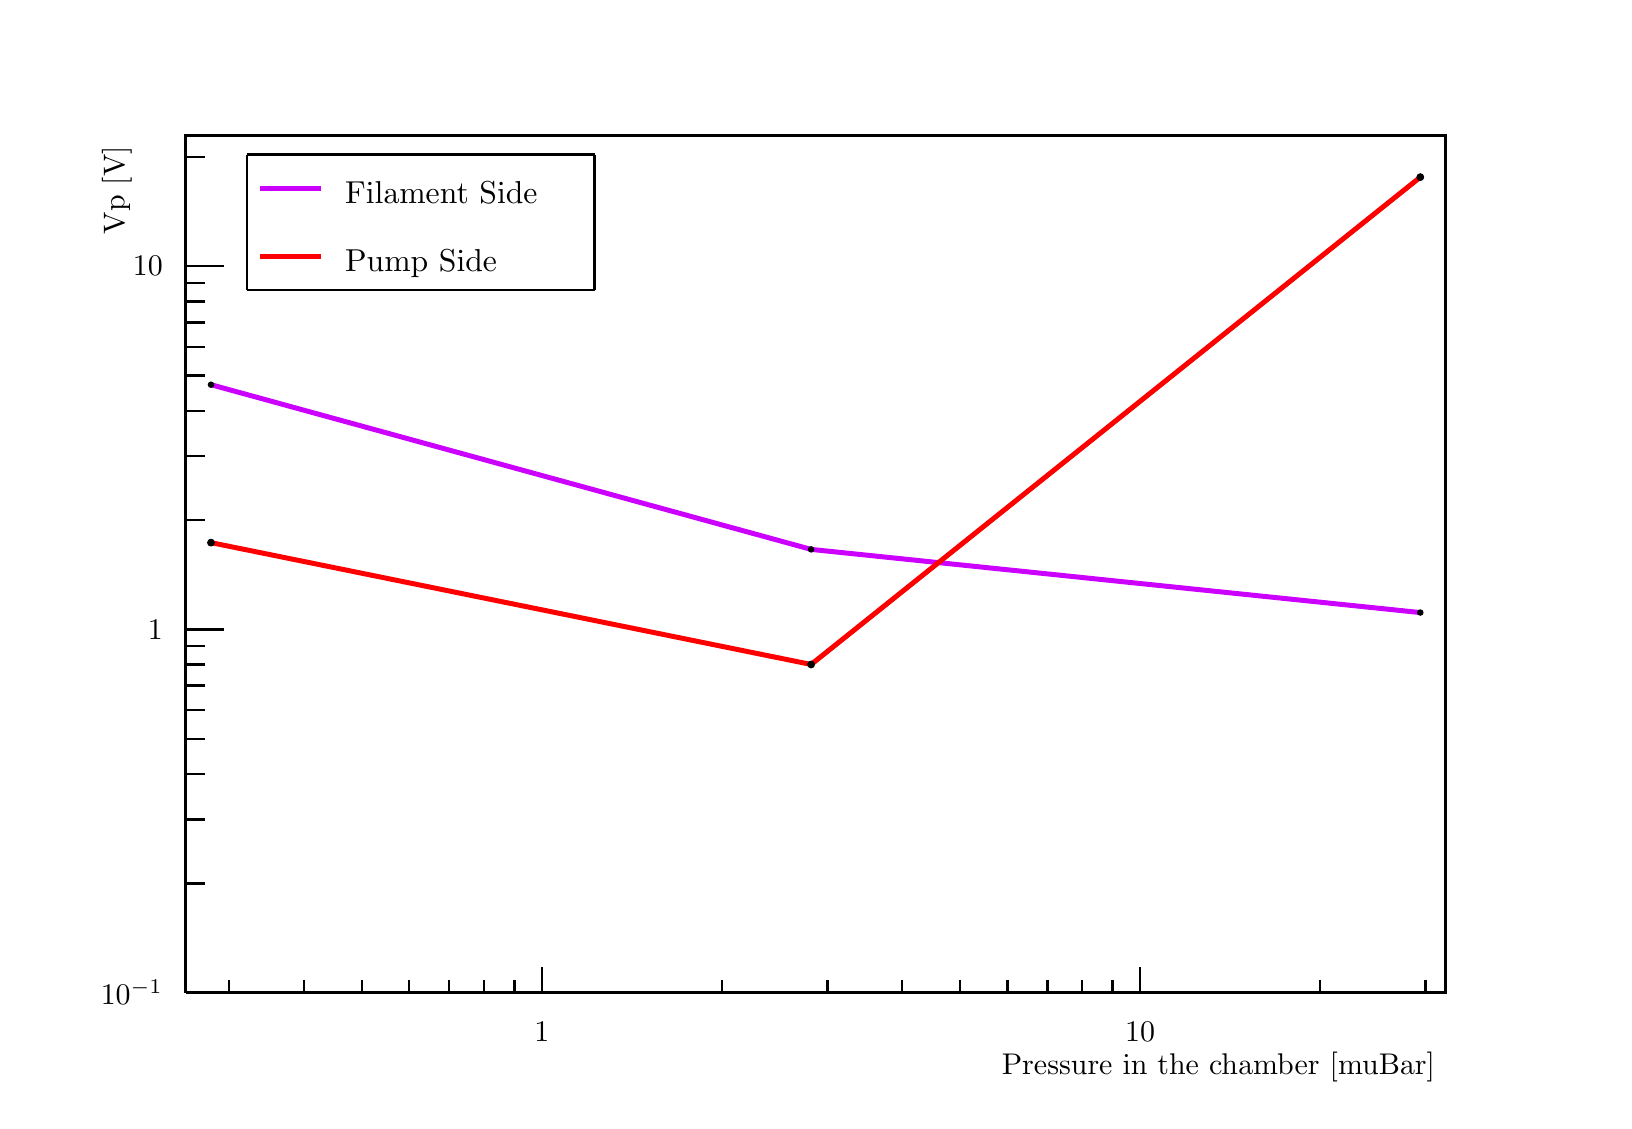
\begin{tikzpicture}
\pgfdeclareplotmark{cross} {
\pgfpathmoveto{\pgfpoint{-0.3\pgfplotmarksize}{\pgfplotmarksize}}
\pgfpathlineto{\pgfpoint{+0.3\pgfplotmarksize}{\pgfplotmarksize}}
\pgfpathlineto{\pgfpoint{+0.3\pgfplotmarksize}{0.3\pgfplotmarksize}}
\pgfpathlineto{\pgfpoint{+1\pgfplotmarksize}{0.3\pgfplotmarksize}}
\pgfpathlineto{\pgfpoint{+1\pgfplotmarksize}{-0.3\pgfplotmarksize}}
\pgfpathlineto{\pgfpoint{+0.3\pgfplotmarksize}{-0.3\pgfplotmarksize}}
\pgfpathlineto{\pgfpoint{+0.3\pgfplotmarksize}{-1.\pgfplotmarksize}}
\pgfpathlineto{\pgfpoint{-0.3\pgfplotmarksize}{-1.\pgfplotmarksize}}
\pgfpathlineto{\pgfpoint{-0.3\pgfplotmarksize}{-0.3\pgfplotmarksize}}
\pgfpathlineto{\pgfpoint{-1.\pgfplotmarksize}{-0.3\pgfplotmarksize}}
\pgfpathlineto{\pgfpoint{-1.\pgfplotmarksize}{0.3\pgfplotmarksize}}
\pgfpathlineto{\pgfpoint{-0.3\pgfplotmarksize}{0.3\pgfplotmarksize}}
\pgfpathclose
\pgfusepathqstroke
}
\pgfdeclareplotmark{cross*} {
\pgfpathmoveto{\pgfpoint{-0.3\pgfplotmarksize}{\pgfplotmarksize}}
\pgfpathlineto{\pgfpoint{+0.3\pgfplotmarksize}{\pgfplotmarksize}}
\pgfpathlineto{\pgfpoint{+0.3\pgfplotmarksize}{0.3\pgfplotmarksize}}
\pgfpathlineto{\pgfpoint{+1\pgfplotmarksize}{0.3\pgfplotmarksize}}
\pgfpathlineto{\pgfpoint{+1\pgfplotmarksize}{-0.3\pgfplotmarksize}}
\pgfpathlineto{\pgfpoint{+0.3\pgfplotmarksize}{-0.3\pgfplotmarksize}}
\pgfpathlineto{\pgfpoint{+0.3\pgfplotmarksize}{-1.\pgfplotmarksize}}
\pgfpathlineto{\pgfpoint{-0.3\pgfplotmarksize}{-1.\pgfplotmarksize}}
\pgfpathlineto{\pgfpoint{-0.3\pgfplotmarksize}{-0.3\pgfplotmarksize}}
\pgfpathlineto{\pgfpoint{-1.\pgfplotmarksize}{-0.3\pgfplotmarksize}}
\pgfpathlineto{\pgfpoint{-1.\pgfplotmarksize}{0.3\pgfplotmarksize}}
\pgfpathlineto{\pgfpoint{-0.3\pgfplotmarksize}{0.3\pgfplotmarksize}}
\pgfpathclose
\pgfusepathqfillstroke
}
\pgfdeclareplotmark{newstar} {
\pgfpathmoveto{\pgfqpoint{0pt}{\pgfplotmarksize}}
\pgfpathlineto{\pgfqpointpolar{44}{0.5\pgfplotmarksize}}
\pgfpathlineto{\pgfqpointpolar{18}{\pgfplotmarksize}}
\pgfpathlineto{\pgfqpointpolar{-20}{0.5\pgfplotmarksize}}
\pgfpathlineto{\pgfqpointpolar{-54}{\pgfplotmarksize}}
\pgfpathlineto{\pgfqpointpolar{-90}{0.5\pgfplotmarksize}}
\pgfpathlineto{\pgfqpointpolar{234}{\pgfplotmarksize}}
\pgfpathlineto{\pgfqpointpolar{198}{0.5\pgfplotmarksize}}
\pgfpathlineto{\pgfqpointpolar{162}{\pgfplotmarksize}}
\pgfpathlineto{\pgfqpointpolar{134}{0.5\pgfplotmarksize}}
\pgfpathclose
\pgfusepathqstroke
}
\pgfdeclareplotmark{newstar*} {
\pgfpathmoveto{\pgfqpoint{0pt}{\pgfplotmarksize}}
\pgfpathlineto{\pgfqpointpolar{44}{0.5\pgfplotmarksize}}
\pgfpathlineto{\pgfqpointpolar{18}{\pgfplotmarksize}}
\pgfpathlineto{\pgfqpointpolar{-20}{0.5\pgfplotmarksize}}
\pgfpathlineto{\pgfqpointpolar{-54}{\pgfplotmarksize}}
\pgfpathlineto{\pgfqpointpolar{-90}{0.5\pgfplotmarksize}}
\pgfpathlineto{\pgfqpointpolar{234}{\pgfplotmarksize}}
\pgfpathlineto{\pgfqpointpolar{198}{0.5\pgfplotmarksize}}
\pgfpathlineto{\pgfqpointpolar{162}{\pgfplotmarksize}}
\pgfpathlineto{\pgfqpointpolar{134}{0.5\pgfplotmarksize}}
\pgfpathclose
\pgfusepathqfillstroke
}
\definecolor{c}{rgb}{1,1,1};
\draw [color=c, fill=c] (0,0) rectangle (20,13.6103);
\draw [color=c, fill=c] (2,1.36103) rectangle (18,12.2493);
\definecolor{c}{rgb}{0,0,0};
\draw [c,line width=0.9] (2,1.36103) -- (2,12.2493) -- (18,12.2493) -- (18,1.36103) -- (2,1.36103);
\definecolor{c}{rgb}{1,1,1};
\draw [color=c, fill=c] (2,1.36103) rectangle (18,12.2493);
\definecolor{c}{rgb}{0,0,0};
\draw [c,line width=0.9] (2,1.36103) -- (2,12.2493) -- (18,12.2493) -- (18,1.36103) -- (2,1.36103);
\draw [c,line width=0.9] (2,1.36103) -- (18,1.36103);
\draw [c,line width=0.9] (2.55171,1.52436) -- (2.55171,1.36103);
\draw [c,line width=0.9] (3.50076,1.52436) -- (3.50076,1.36103);
\draw [c,line width=0.9] (4.23689,1.52436) -- (4.23689,1.36103);
\draw [c,line width=0.9] (4.83836,1.52436) -- (4.83836,1.36103);
\draw [c,line width=0.9] (5.34689,1.52436) -- (5.34689,1.36103);
\draw [c,line width=0.9] (5.78741,1.52436) -- (5.78741,1.36103);
\draw [c,line width=0.9] (6.17597,1.52436) -- (6.17597,1.36103);
\draw [c,line width=0.9] (6.52354,1.68768) -- (6.52354,1.36103);
\draw [anchor=base] (6.52354,0.745165) node[scale=1.08185, color=c, rotate=0]{1};
\draw [c,line width=0.9] (8.81019,1.52436) -- (8.81019,1.36103);
\draw [c,line width=0.9] (10.1478,1.52436) -- (10.1478,1.36103);
\draw [c,line width=0.9] (11.0968,1.52436) -- (11.0968,1.36103);
\draw [c,line width=0.9] (11.833,1.52436) -- (11.833,1.36103);
\draw [c,line width=0.9] (12.4345,1.52436) -- (12.4345,1.36103);
\draw [c,line width=0.9] (12.943,1.52436) -- (12.943,1.36103);
\draw [c,line width=0.9] (13.3835,1.52436) -- (13.3835,1.36103);
\draw [c,line width=0.9] (13.7721,1.52436) -- (13.7721,1.36103);
\draw [c,line width=0.9] (14.1196,1.68768) -- (14.1196,1.36103);
\draw [anchor=base] (14.1196,0.745165) node[scale=1.08185, color=c, rotate=0]{10};
\draw [c,line width=0.9] (16.4063,1.52436) -- (16.4063,1.36103);
\draw [c,line width=0.9] (17.7439,1.52436) -- (17.7439,1.36103);
\draw [anchor= east] (18,0.415931) node[scale=1.08185, color=c, rotate=0]{Pressure in the chamber [muBar]};
\draw [c,line width=0.9] (2,1.36103) -- (2,12.2493);
\draw [c,line width=0.9] (2.48,1.36235) -- (2,1.36235);
\draw [anchor= east] (1.844,1.36235) node[scale=1.08185, color=c, rotate=0]{$10^{-1}$};
\draw [c,line width=0.9] (2.24,2.7509) -- (2,2.7509);
\draw [c,line width=0.9] (2.24,3.56314) -- (2,3.56314);
\draw [c,line width=0.9] (2.24,4.13944) -- (2,4.13944);
\draw [c,line width=0.9] (2.24,4.58645) -- (2,4.58645);
\draw [c,line width=0.9] (2.24,4.95168) -- (2,4.95168);
\draw [c,line width=0.9] (2.24,5.26048) -- (2,5.26048);
\draw [c,line width=0.9] (2.24,5.52798) -- (2,5.52798);
\draw [c,line width=0.9] (2.24,5.76393) -- (2,5.76393);
\draw [c,line width=0.9] (2.48,5.97499) -- (2,5.97499);
\draw [anchor= east] (1.844,5.97499) node[scale=1.08185, color=c, rotate=0]{1};
\draw [c,line width=0.9] (2.24,7.36353) -- (2,7.36353);
\draw [c,line width=0.9] (2.24,8.17578) -- (2,8.17578);
\draw [c,line width=0.9] (2.24,8.75207) -- (2,8.75207);
\draw [c,line width=0.9] (2.24,9.19908) -- (2,9.19908);
\draw [c,line width=0.9] (2.24,9.56432) -- (2,9.56432);
\draw [c,line width=0.9] (2.24,9.87312) -- (2,9.87312);
\draw [c,line width=0.9] (2.24,10.1406) -- (2,10.1406);
\draw [c,line width=0.9] (2.24,10.3766) -- (2,10.3766);
\draw [c,line width=0.9] (2.48,10.5876) -- (2,10.5876);
\draw [anchor= east] (1.844,10.5876) node[scale=1.08185, color=c, rotate=0]{10};
\draw [c,line width=0.9] (2.24,11.9762) -- (2,11.9762);
\draw [anchor= east] (1.1264,12.2493) node[scale=1.08185, color=c, rotate=90]{Vp [V]};
\definecolor{c}{rgb}{0.8,0,1};
\draw [c,line width=1.8] (2.32092,9.08309) -- (9.94269,6.9914) -- (17.6791,6.18911);
\definecolor{c}{rgb}{0,0,0};
\foreach \P in {(2.32092,9.08309), (9.94269,6.9914), (17.6791,6.18911)}{\draw[mark options={color=c,fill=c},mark size=0.960961pt,mark=*] plot coordinates {\P};}
\definecolor{c}{rgb}{1,0,0};
\draw [c,line width=1.8] (2.32092,7.07736) -- (9.94269,5.53009) -- (17.6791,11.7192);
\definecolor{c}{rgb}{0,0,0};
\foreach \P in {(2.32092,7.07736), (9.94269,5.53009), (17.6791,11.7192)}{\draw[mark options={color=c,fill=c},mark size=1.201201pt,mark=*] plot coordinates {\P};}
\definecolor{c}{rgb}{1,1,1};
\draw [color=c, fill=c] (2.77937,10.2865) rectangle (7.19198,12.0057);
\definecolor{c}{rgb}{0,0,0};
\draw [c,line width=0.9] (2.77937,10.2865) -- (7.19198,10.2865);
\draw [c,line width=0.9] (7.19198,10.2865) -- (7.19198,12.0057);
\draw [c,line width=0.9] (7.19198,12.0057) -- (2.77937,12.0057);
\draw [c,line width=0.9] (2.77937,12.0057) -- (2.77937,10.2865);
\draw [anchor=base west] (3.88252,11.3825) node[scale=1.14549, color=c, rotate=0]{Filament Side};
\definecolor{c}{rgb}{0.8,0,1};
\draw [c,line width=1.8] (2.94484,11.5759) -- (3.71705,11.5759);
\definecolor{c}{rgb}{0,0,0};
\draw [anchor=base west] (3.88252,10.5229) node[scale=1.14549, color=c, rotate=0]{Pump Side};
\definecolor{c}{rgb}{1,0,0};
\draw [c,line width=1.8] (2.94484,10.7163) -- (3.71705,10.7163);
\end{tikzpicture}
